\documentclass[11pt, aspectration=169]{beamer}
\usetheme{Copenhagen}
\usecolortheme{seahorse}
\setbeamertemplate{headline}{}
\usepackage{graphicx} % Required for inserting images
\usepackage{amsmath, amssymb, amsthm}
\usepackage{ragged2e}

\title{Predstavitev 1. domače naloge, NRO}
\author{Luka Michael Gradišek, 23221005}
\date{November 2024}

\begin{document}

\maketitle

\begin{frame}{Kazalo}
\tableofcontents
\end{frame}

\section{Predstavitev prve naloge}
\begin{frame}{Predstavitev prve naloge}
\justifying
V prvi nalogi prebiramo podatke iz tekstovne datoteke \textit{naloga1\_1.txt}. Prva vrstica datoteke vsebuje ime parametra, ki ga analiziramo, v našem primeru je to čas (\textit{time [s]}). Druga vrstica določa število vrstic in število podatkov v vsaki vrstici. Datoteka vsebuje 100 vrstic, vsaka pa vsebuje po en podatek, kar pomeni, da imamo na voljo 100 vrednosti časa, podanih v sekundah. Te vrednosti moramo uvoziti v \textbf{MATLAB} in jih shraniti v vektor.

Za branje podatkov uporabimo funkcijo \textit{importdata}. Funkciji predamo ime datoteke (\textit{naloga1\_1.txt}) kot prvi parameter. 
Kot drugi parameter določimo ločilo (\textit{delimiterIn}), ki funkciji pove, kako so podatki ločeni. 
Tretji parameter, \textit{headerlinesIn}, pa pove, koliko začetnih vrstic je treba preskočiti, preden funkcija začne brati podatke. 
Časovne vrednosti nato preprosto shranimo v vektor $t$ z ukazom 

\texttt{t = data.data(:, 1)}.
\end{frame}

\section{Graf P(t)}
\begin{frame}{Graf moči v odvisnosti od časa}
Na spodnjem grafu \ref{fig:Graf P(t)} imamo prikazano odvisnost moči od časa iz katerega opazimo, da le ta s časom pada.
\begin{figure}
    \centering
    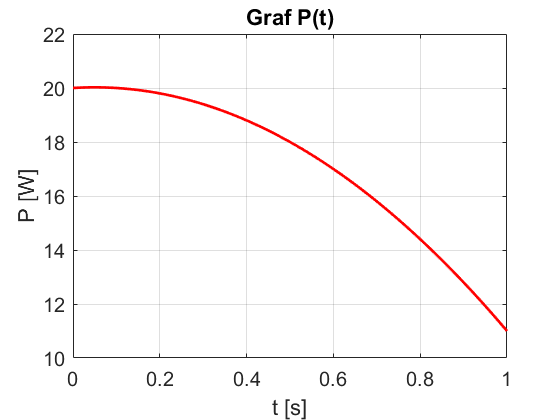
\includegraphics[width=0.65\textwidth]{graf1.png}
    \caption{Graf P(t)}
    \label{fig:Graf P(t)}
\end{figure}
    
\end{frame}

\section{Numerično integriranje}
\begin{frame}{Numerično integriranje s trapezno metodo}
Integral smo izračunali tako z že vgrajeno funkcijo \textit{trapz} in z teoretično formulo integrala. Nato pa smo obe vrednosti odšteli in tako izračunali razliko med njima.
\begin{block}{Formula za \textit{trapz} metodo}
\small
\[
\int_{a}^{b} f(x) dx = \frac{\Delta x}{2} \left( f(x_0) + 2f(x_1) + 2f(x_2) + \dots + 2f(x_{n-1}) + f(x_n) \right)
\]
\end{block}
\begin{block}{Rešitev po teoretični formuli}
Zgornja formula nam poda vrednost: 
\[
\int_{t_{min}}^{t_{max}} P(t) dt = \int_{0}^{1} P(t) dt = 17.1665
\]
\end{block}

\end{frame}

\end{document}
